\section{Análise experimental}
\label{sec:imageblur/experimental}

Os gráficos seguintes foram gerados usando a biblioteca \textit{matplotlib} do \textit{python}. Para gerar os gráficos foram primeiro gerados ficheiros com os dados obtidos através da biblioteca \textit{time} da linguagem C. Depois foram gerados os gráficos a partir desses ficheiros. Para cada gráfico foram usados 12100 resultados.

\subsection{Primeira abordagem}

\begin{figure}[H]
    \centering
    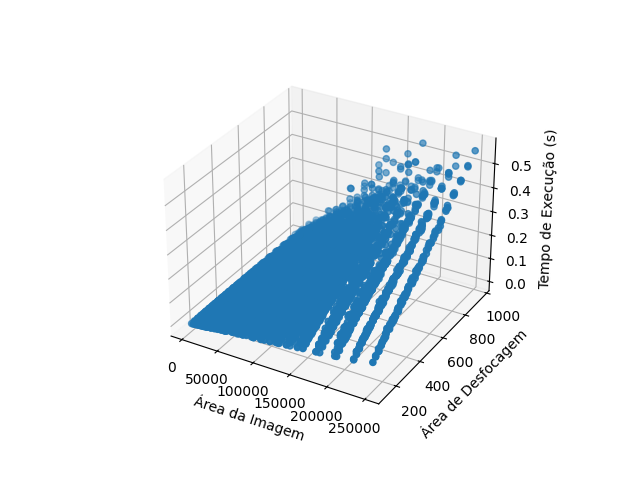
\includegraphics[width=\linewidth]{images/first-3d_plot.png}
    \caption{Gráfico 3D do tempo de execução da primeira abordagem.}
    \label{fig:imageblur/first-3d_plot}
\end{figure}

Como podemos ver na figura \ref{fig:imageblur/first-3d_plot}, o tempo de execução da primeira abordagem é linear em função do tamanho da imagem e linear em função da área de desfocagem o que implica que o total seja exponencial em função de ambos. Isto para valores pequenos pode não se notar muito mas à medida que queremos trabalhar com imagems maiores ou filtros maiores, este algoritmo torna-se inviável.

\subsection{Segunda abordagem}

\begin{figure}[H]
    \centering
    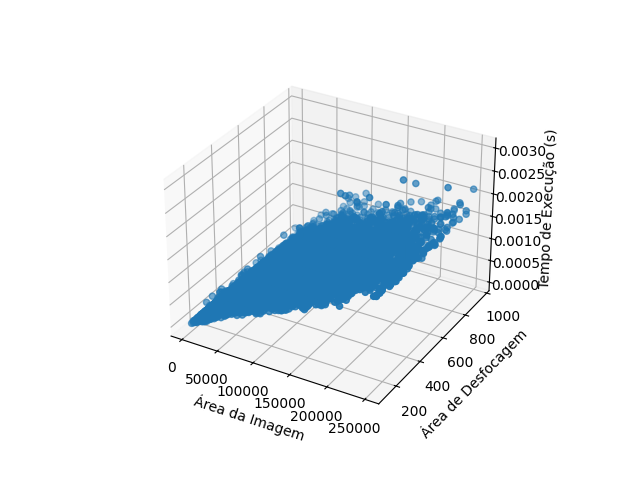
\includegraphics[width=\linewidth]{images/second-3d_plot.png}
    \caption{Gráfico 3D do tempo de execução da segunda abordagem.}
    \label{fig:imageblur/second-3d_plot}
\end{figure}

Como podemos ver na figura \ref{fig:imageblur/second-3d_plot}, o tempo de execução da segunda abordagem é linear em função do tamanho da imagem. Podemos também ver que a área de desfocagem não tem influência no tempo de execução. Isto permite conseguir trabalhar com imagens maiores sem ter problemas com ineficiência do programa bem como usar qualquer tamanho de filtro sem alterar de forma alguma o desempenho do programa.

\subsection{Comparação}

Como se pode concluir a partir dos gráficos anteriores, a segunda abordagem é muito mais eficiente que a primeira. O pricipal motivo para isso é que, embora ambas as abordagens usem os mesmos ciclos principais, na primeira abordagem esse ciclo contém ainda um segundo dentro dele, o que vai fazer com que o tempo execução para o mesmo tamanho de imagem seja sempre superior ao da segunda abordagem visto que o tempo da primeira é sempre incrementado pelo tamanho do filtro coisa que não acontece com o segundo algoritmo.

